\documentclass[a4paper, 14pt]{extarticle}

\usepackage[T2A]{fontenc}
\usepackage{natbib}
\usepackage{graphicx}
\usepackage[english, russian]{babel}
\usepackage{fontspec}
\usepackage{amsmath}
\usepackage{amsfonts}
\usepackage{amssymb}
\usepackage{amsthm}
\usepackage{mathtools}
\usepackage{mathrsfs}
\usepackage{icomma}
\usepackage{fullpage}
\usepackage{ulem}
\usepackage{setspace}
\usepackage{listings}
\usepackage{indentfirst}
\usepackage[left=2cm,right=1.5cm,top=2cm,bottom=2cm]{geometry}
\usepackage{xcolor}
\usepackage{float}
\usepackage{csquotes}
\usepackage{hyperref}
\usepackage{graphics}



\definecolor{urlcolor}{HTML}{0000FF} % цвет гиперссылок
\definecolor{linkcolor}{HTML}{000000} % цвет гиперссылок
\hypersetup{pdfstartview=FitH, linkcolor=linkcolor, urlcolor=urlcolor, colorlinks=true}


\setmainfont{Times New Roman}
\setlength{\parindent}{5ex}
\setlength{\parskip}{1em}
\renewcommand{\baselinestretch}{1}

\graphicspath{{images/}}


\definecolor{buzzlightyear}{HTML}{8757A5}
\definecolor{grass}{HTML}{738D06}
\definecolor{literal}{HTML}{F18A2B}
\definecolor{commentcolor}{HTML}{8E908B}

\lstdefinestyle{habrstyle}{
    backgroundcolor=\color{white},
    commentstyle=\color{commentcolor},
    keywordstyle=\bfseries\color{buzzlightyear},
    numberstyle=\tiny\color{commentcolor},
    stringstyle=\color{grass},
    basicstyle=\ttfamily\footnotesize,
    breakatwhitespace=false,
    breaklines=true,
    captionpos=b,
    keepspaces=true,
    numbers=left,
    numbersep=5pt,
    showspaces=false,
    showstringspaces=false,
    showtabs=false,
    tabsize=4
}

\lstset{style=habrstyle}

\begin{document}
    % НАЧАЛО ТИТУЛЬНОГО ЛИСТА
    \begin{center}
        \begin{center}
            \hfill \break
            \normalsize{Санкт-Петербургский государственный политехнический}\\
            \normalsize{университет Петра Великого}\\
            \hfill \break
            \normalsize{\textbf{Высшая школа интеллектуальных систем и}}\\
            \normalsize{\textbf{суперкомпьютерных технологий}}\\
            \hfill \break
            \hfill \break
            \hfill \break
            \normalsize{Лабораторная работа}\\
            \hfill \break
            \normalsize{\LARGE Модуляция и выборка (квантование)}\\
        \end{center}
        \hfill \break
        \hfill \break
        \hfill \break
        \hfill \break
        \hfill \break
        \hfill \break
        \hfill \break
        \hfill \break
        \hfill \break
        \hfill \break
        \begin{tabbing}
            Выполнил студент гр. 3530901/80201 \`И.С. Иванов\\
            \\
            Преподаватель: \`Н.В. Богач\\
        \end{tabbing}
        \hfill \break
        \hfill \break
        \hfill \break
        \hfill \break
        \begin{center}
            Санкт-Петербург\\
            2021
        \end{center}
        \thispagestyle{empty}
    \end{center}
    % КОНЕЦ ТИТУЛЬНОГО ЛИСТА

    % ОГЛАВЛЕНИЕ
    \newpage
    \tableofcontents

    % СПИСОК ИЛЛЮСТРАЦИЙ
    \newpage
    \listoffigures

    % СПИСОК ЛИСТИНГОВ
    \newpage
    \lstlistoflistings

    \newpage


    \section{Упражнение №1}
    \label{sec:1}

    В первом упражнении необходимо изучить примеры из файла \texttt{chap11.ipynb}.

    Все примеры были запущены и изучены.

    \newpage


    \section{Упражнение №2}
    \label{sec:2}

    В втором упражнении необходимо просмотреть ролик Криса "Монти" Минтгомери - "D/A and A/D | Digital Show and Tell".

    В результате просмотра данного видеоролика была получена информация, почему аналоговое аудио в приемлемых пределах человеческого слуха воспроизводится с идеальной точностью с использованием 16-битного цифрового сигнала 44.1 кГЦ.

    \newpage


    \section{Упражнение №3}
    \label{sec:3}

    В третьем упражнении необходимо применить фильтр низких частот к примеру "Соло на барабане" до выборки.
    После чего снова с помощью фильтра НЧ удалить спектральные копии, которые вызваны выборкой.

    Считаем файл.

    \begin{lstlisting}[language=Python, caption= Считывание сигнала, label={lst:read_wave}]
        from thinkdsp import read_wave

        wave = read_wave('Sounds/263868__kevcio__amen-break-a-160-bpm.wav')
        wave.normalize()
        wave.plot()
    \end{lstlisting}

    \begin{figure}[H]
        \centering
        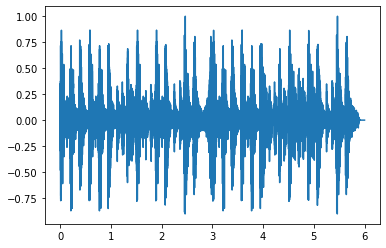
\includegraphics[width=0.8\linewidth]{drum_wave}
        \caption{Полученный сигнал}
        \label{fig:drum_wave}
    \end{figure}

    Получим спектр.

    \begin{figure}[H]
        \centering
        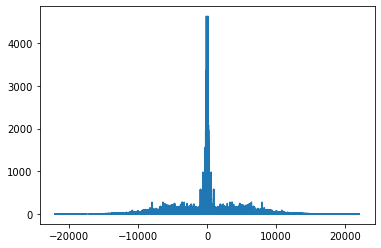
\includegraphics[width=0.8\linewidth]{drum_spectrum}
        \caption{Спектр сигнала}
        \label{fig:drum_spectrum}
    \end{figure}

    Уменьшим частоту дискретизации в 3 раза.

    \begin{lstlisting}[language=Python, caption= Уменьшение частоты дискретизации, label={lst:downsampling}]
        factor = 3
        framerate = wave.framerate / factor
        cutoff = framerate / 2 - 1
    \end{lstlisting}

    Применим фильтр сглаживания для удаления частот выше новой частоты.

    \begin{lstlisting}[language=Python, caption= Применение фильтра, label={lst:apply_filter}]
        spectrum.low_pass(cutoff)
        spectrum.plot()
    \end{lstlisting}

    \begin{figure}[H]
        \centering
        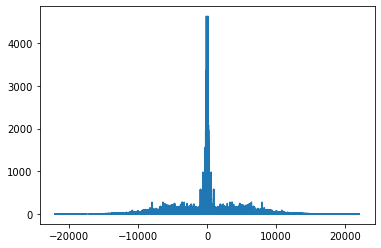
\includegraphics[width=0.8\linewidth]{drum_after_filter}
        \caption{Применение фильтра}
        \label{fig:drum_after_filter}
    \end{figure}

    Теперь напишем функцию \texttt{sample}, которая будет имитировать процесс выборки.

    \begin{lstlisting}[language=Python, caption= Функция sample, label={lst:sample}]
        from thinkdsp import Wave

        def sample(wave, factor):
            ys = np.zeros(len(wave))
            ys[::factor] = np.real(wave.ys[::factor])
            return Wave(ys, framerate=wave.framerate)
    \end{lstlisting}

    Проверим функцию.

    \begin{lstlisting}[language=Python, caption= Применения sample, label={lst:apply_sample}]
        filtered = spectrum.make_wave()
        sampled = sample(filtered, factor)
        sampled_spectrum = sampled.make_spectrum(full=True)
        sampled_spectrum.plot()
    \end{lstlisting}

    \begin{figure}[H]
        \centering
        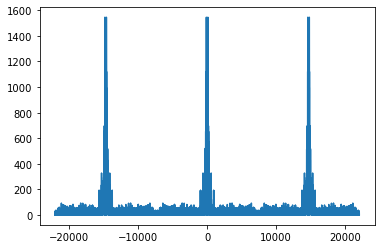
\includegraphics[width=0.8\linewidth]{drum_sample}
        \caption{Применение функции sample}
        \label{fig:drum_sample}
    \end{figure}

    На спектре имеются спектральные копии.
    Необходимо убрать их применив фильтр сглаживания.

    \begin{figure}[H]
        \centering
        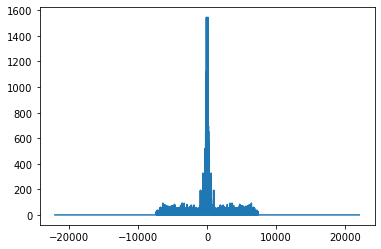
\includegraphics[width=0.8\linewidth]{drum_sample_after_filter}
        \caption{Применения сглаживания}
        \label{fig:drum_sample_after_filter}
    \end{figure}

    Масштабируем спектр.

    \begin{figure}[H]
        \centering
        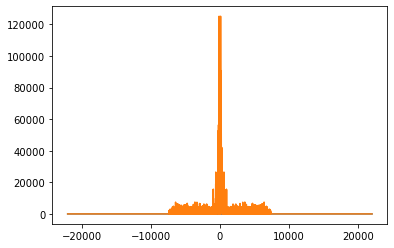
\includegraphics[width=0.8\linewidth]{drum_zoomed}
        \caption{Масштабирование спектра}
        \label{fig:drum_zoomed}
    \end{figure}

    Проверим разницу между спектром до и после фильтрации.

    Между спектрами нет большой разницы.
    Функция \texttt{max\_diff} выводит результат 1.8189894035458565e-12, подтверждая это.

    Посмотрим на сигнал.

    \begin{figure}[H]
        \centering
        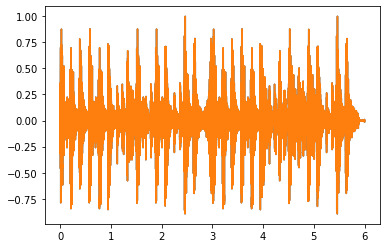
\includegraphics[width=0.8\linewidth]{result}
        \caption{Результат}
        \label{fig:result}
    \end{figure}

    По полученным результатам можно сделать вывод, что разница между интерполированной и фильтрованной волной очень мала.

    \newpage


    \section{Выводы}
    \label{sec:conclusions}

    В результате выполнения данной лабораторной работы были получены знания об амплитудной модуляции.
    Амплитудная модуляция играет важную роль в радиосвязи.
    Также была изучена теорема о выборках, которая является важнейшей в цифровой обработке сигналов.
    Также были получены навыки их применения.

\end{document}